\documentclass[JCDReport.tex]{subfiles} 
\begin{document}

\subsection{Code Coverage}

To measure the code coverage of the VFSBase and VFSBaseTests correctly, the DiskServiceReference has to be excluded from the coverage, because this code is generated automatically and therefore is irrelevant for the test coverage (WCF service reference). Figure \ref{fig:excludeTests} shows how this is done for the VFSBase project.\\

\begin{figure}[h!]
	\centering
	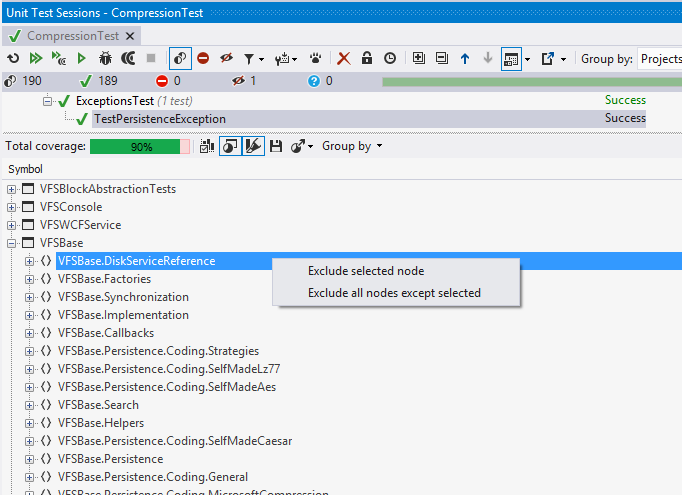
\includegraphics[scale=0.75]{Images/code_coverage1.png} 
	\caption{WCFService dependency diagram}
	\label{fig:excludeTests}
\end{figure}	

The code coverage of the code was at 94\% on Monday, 2013-05-13 at 4.46 pm, see Figure \ref{fig:codeCoverage}.

\begin{figure}[h!]
	\centering
	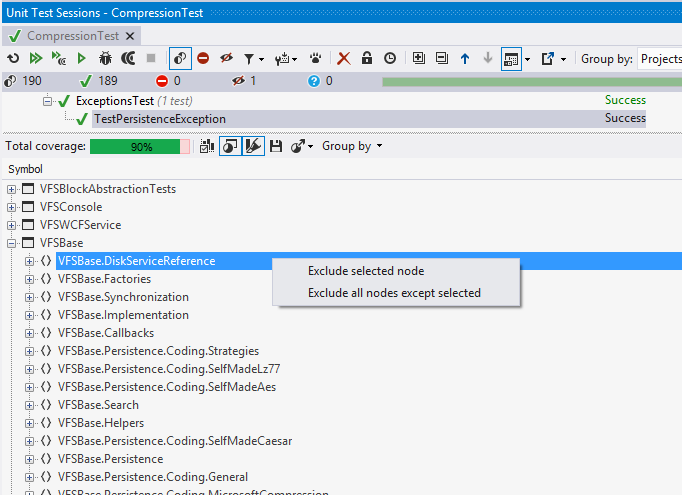
\includegraphics[scale=0.75]{Images/code_coverage1.png} 
	\caption{WCFService dependency diagram}
	\label{fig:codeCoverage}
\end{figure}	

\end{document}

